\documentclass[a4paper]{exam}

\usepackage{graphicx}
\usepackage{pgfplots}
\pgfplotsset{compat=1.11}

\usepackage{siunitx}
\DeclareSIUnit{\revolution}{rev}
\DeclareSIUnit{\rpm}{\revolution\per\minute}
\DeclareSIUnit{\lightyear}{ly}

\begin{document}
  \section*{L2 Physics: Problems on mechanics}
  See the final page for useful formulae and constants.
  \subsection*{Sections 2.1-2.2}
  Main concepts you should understand: vector, displacement, velocity, acceleration
  \begin{questions}
    \question Below are drawn vectors $ \vec{a} $ and $ \vec{b} $. Draw (a) $ \vec{a} + \vec{b} $; (b) $ \vec{a} - \vec{b} $.

      \begin{tikzpicture}
        \begin{axis}[axis lines = center, xmin=-5,xmax=5,ymin=-5,ymax=5]
          \draw[->] (0,0) --  (3,2) node[above]{$\vec{a}$};
          \draw[->] (0,0) --  (-1,4) node[above]{$\vec{b}$};
        \end{axis}
      \end{tikzpicture}
    \question A car decelerates from $ \vec{v}_0 = \SI{5}{\metre\per\second} $ to $ \vec{v}_1 = \SI{1}{\metre\per\second} $.
              Draw a vector diagram depicting the two velocity vectors, and the change in velocity.
    \question Suppose one starts from point $ A $ and walks south \SI{230}{\metre} and then walks \SI{350}{\metre}
              west of north to a point $ B $. Find the distance from $ A $ to $ B $ as the crow flies.
    \question A runner runs \SI{3400}{\metre} in 10 minutes and 33 seconds; what was her average speed in metres per second?
    \question A car moving at \SI{25}{\metre\per\second} stops suddenly in \SI{14.0}{\second}. What was average acceleration
              of the car during this time, and how far did the car travel before stopping?
    \question A bullet moving at a speed of \SI{150}{\metre\per\second} travels \SI{3.5}{\centi\metre} into a block of glass
              before stopping. Find the average acceleration of the bullet, and the time taken for it to stop.
    \question A stone is thrown straight upwards from the ground, and goes as high as a nearby building. The stone
              reaches the ground \SI{3.0}{\second} after it is thrown. How tall is the building?
    \question A piano is pushed out of a window that is \SI{8}{\metre} above a person sitting below. How
              fast is it moving when it hits the person, and how long do they have to get out of the way?
    \question A train blocks a crossing; it takes \SI{20}{\second} for a carriage to pass through a distance
              equal to the length of one carriage as the train starts to move. Assuming the length of a carriage is $ L $
              and the acceleration of the train is constant, how long will it take for the next twenty railway carriages
              to pass by?
    \question A car is moving at \SI{30}{\metre\per\second}. Assuming an average deceleration of \SI{7.0}{\metre\per\second\per\second},
              how long will it take for the car to stop?
    \question A ball is thrown straight upwards with a speed $ v $ from a point $ h $ metres above the ground. Show that the time
              taken for the ball to strike the ground is
              \[ \frac{v}{g}\left( 1 + \sqrt{1 + \frac{2hg}{v^2}} \right). \]
  \end{questions}
  \subsection*{Section 2.3}
  Main concepts you should understand: force, torque, acceleration, equilibrium
  \begin{questions}
    \question A \SI{7.0}{\gram} bullet is given an acceleration of \SI{40,000}{\metre\per\second\per\second} as it is shot from
              a gun with a \SI{6.0}{\centi\metre} barrel. How large is the average force on the bullet during this process?
    \question How much force does an \SI{70}{\kilo\gram} person exert on the earth due to gravity?
    \question A \SI{1300}{\kilo\gram} car must be stpped in a distance of \SI{80}{\metre}. The initial speed of the car
              is \SI{20}{\metre\per\second}. What force needs to be exerted, assuming constant deceleration?
    \question (NZQA 2012) Hannah (55 kg) stands on a see-saw. The see-saw has a weight of \SI{210}{\newton}. Calculate the
              size and direction of the force that the floor exerts on the right hand end of the see-saw.

              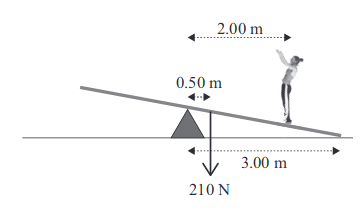
\includegraphics[width=0.4\textwidth]{nzqa20121}
    \question (NZQA 2013) Jason is at a fair of some description.
      \begin{parts}
        \part Jason goes for a ride on a go-kart. Towards the end of the ride, he decelerates at \SI{2.5}{\metre\per\second\per\second}
              and comes to a stop in 4.2 seconds.  By calculating Jason’s initial velocity, determine the distance he travels
              while coming to a stop.
        \part Jason sits on a slide. He is sliding down at constant speed.

              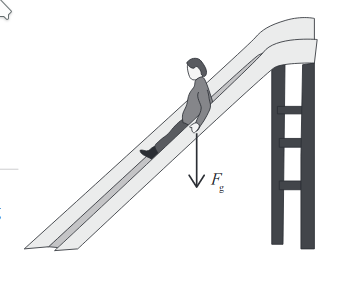
\includegraphics[width=0.4\textwidth]{nzqa20131}
          \begin{subparts}
            \subpart State the size of the net force on Jason. Explain your answer.
            \subpart On the diagram on the right, draw the remaining
                     forces (as labelled vectors) acting on Jason.
            \subpart Complete and label the vector addition
                     diagram of the forces acting on Jason.
          \end{subparts}
      \end{parts}
    \question (NZQA 2013) The diagram below represents a see-saw on a pivot at its centre with Jane and her dad sitting on
              opposite sides such that the see-saw is in equilibrium. The mass of the see-saw itself is \SI{60}{\kilo\gram}.

              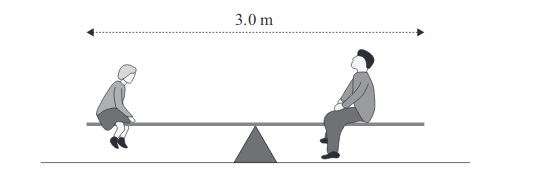
\includegraphics[width=0.4\textwidth]{nzqa201321}
      \begin{parts}
        \part On the diagram above, draw labelled vectors to show all the forces acting on the see-saw.
        \part Jane and her dad move to opposite ends of the see-saw.
              The diagram below shows what happens when Jane sits at one end of the see-saw while her
              dad sits at the other end.

              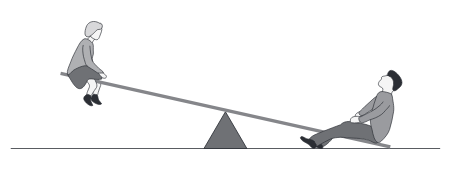
\includegraphics[width=0.4\textwidth]{nzqa201322}

              If Jane's mass is \SI{30}{\kilo\gram} and Jane's dad's mass is \SI{72}{\kilo\gram}, calculate the
              size of the support force from the ground at the end where Jane's dad is sitting. Round your answer
              to the correct number of significant figures.
      \end{parts}
    \question (NZQA 2012) The Clown makes his entrance riding on a cart pulled by Hannah. The clown and cart have a
              combined mass of \SI{85}{\kilo\gram}. The handle of the cart makes an angle of \ang{30} to the horizontal
              as shown in the diagram below. Hannah applies a force of \SI{55}{\newton} to the handle.

              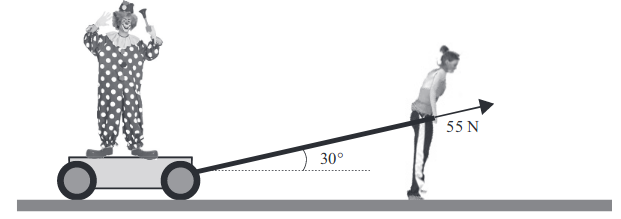
\includegraphics[width=0.4\textwidth]{nzqa20122}

      \begin{parts}
        \part Calculate the size of the horizontal component of the force on the handle.
        \part The cart is in equilibrium.
          \begin{itemize}
            \item State what ``equilibrium'' means in terms of the forces acting on the cart.
            \item Describe what it tells you about the velocity of the cart.
            \item On the diagram above, draw labelled arrows showing the direction of any non-vertical
                  forces acting on Hannah.
          \end{itemize}
        \part Explain how Hannah can make the cart and clown accelerate without changing the size
              of the force she exerts on the handle. (Reducing friction is not a possibility.)
      \end{parts}
    \question A box of mass $ m $ slides down an incline that makes an angle $ \theta $ with the vertical, with an acceleration $ a $.
              A friction force $ f $ impedes its motion. (a) Draw a free body (force) diagram; (b) find the acceleration $ m $
              in terms of $ \theta $, $ m $, and $ f $.
    \question The weight of an object is defined to be the force exerted on it by gravity; so $ W = mg $, where $ m $ is the
              mass of the object. If a three ton (\SI{3000}{\kilo\gram}) car is travelling at \SI{40}{\kilo\metre\per\hour}
              and the brakes are suddenly applied, and it skids to rest, how far does the car skid given that the friction
              force experienced by the tires is around 0.7 times the weight of the car?
    \question Newton's law of gravity tells us that if we have two objects $ A $ and $ B $, with masses $ m_A $ and $ m_b $,
              such that the distance between them is $ r $, then the force that $ A $ exerts on $ B $ due to gravity is
              \begin{displaymath}
                F = \frac{Gm_A m_B}{r^2}.
              \end{displaymath}
              Given that $ F = ma $, the units of force are $ \si{\newton} = \si{\kilo\gram\metre\per\second\per\second} $. What
              are the units of the gravitational constant $ G $?
  \end{questions}
  \section*{Sections 2.4-2.5}
  Main concepts you should understand: momentum, energy (kinetic, gravitational potential, elastic potential), conservation laws of momentum and energy,
  impulse, elastic/inelastic collision.
  \begin{questions}
    \question A \SI{1500}{\kilo\gram} car, travelling at 20 metres per second, reduces its speed over \SI{3.0}{\second}
              to \SI{15}{\metre\per\second}. Calculate the impulse felt by the car. What was the average force causing the deceleration?
    \question Find the momentum of an \SI{800}{\gram} object after it falls freely from rest a height of \SI{60}{\centi\metre}.
    \question A \SI{120}{\gram} ball moving at \SI{18}{\metre\per\second} hits a wall perpendicularly and rebounds with the same
              speed. After intially touching the wall, the centre of the ball moves an extra \SI{0.27}{\centi\metre} towards it
              before rebounding. (a) Assuming constant deceleration, show that the total time the ball is in contact with the
              wall is $ 2 \times 0.00030 \si{\second} $. (b) What is the average force the ball exerts on the wall?
    \question A \SI{60}{\kilo\gram} astronaut becomes seperated from her ship; she is \SI{15.0}{\metre} away and at rest
              relative to it. She throws a \SI{500}{\gram} spanner at a speed of \SI{8.0}{\metre\per\second} in a direction
              away from the ship; how long does it take her to get back to the ship?
    \question An object of mass \SI{2.0}{\kilo\gram} falls, from rest, through a height $ h $. When it reaches the bottom, its
              speed is measured as \SI{4}{\metre\per\second}. Calculate $ h $. How long did the object take to fall through the height?
    \question A \SI{2000}{\kilo\gram} car is travelling at \SI{20}{\metre\per\second} up a frictionless hill when the motor stops. (a) If the car
              is a vertical distance of \SI{8}{\metre} from the top of the hill at that point, will it be able to reach the top? (b) How far below
              the top of the hill could the car be to still reach the top?
    \question What power does a \SI{60}{\kilo\gram} person develop when they lift themselves \SI{12.0}{\metre} in \SI{20.0}{\second} using
              a flight of stairs?
    \question A \SI{20.0}{\kilo\gram} crate is pushed \SI{6.0}{\metre} along the floor at a constant speed by a force
              inclined \ang{30} below the horizontal. (a) Describe the changes of energy occuring as the crate
              moves along the floor. (b) If the friction force retarding the motion is \SI{140}{\newton},
              draw a free body diagram and calculate the net force acting on the crate. (c) How much work is done by
              the pushing force?
    \question (NZQA 2012) Jess is a trapeze artist at the circus. As part of her act she hangs
              on a long rope and swings downwards. When she gets to the lowest point she grabs
              onto Hannah (another performer) and they keep moving together. Jess has a mass of \SI{65}{\kilo\gram};
              Hannah has a mass of \SI{55}{\kilo\gram}.
      \begin{parts}
        \part Name the quantity that is conserved as Jess swings down.
        \part Name the quantity that is conserved as Jess graps Hannah and they swing together.
        \part Immediately after Jess grabs Hannah, they move together at a speed of \SI{5.5}{\metre\per\second}.
              Calculate the vertical height that Jess dropped down.
      \end{parts}
    \question (NZQA 2012) Hannah flies through the air and lands on an elastic rope, which is held
              under tension between two supports.
      \begin{parts}
        \part Name the main energy changes that occur as Hannah is falling AND as she is coming to a stop.
        \part Hannah doesn’t like the rope to be too tight when she lands on it.
              State the direction of the force on her from the rope.
              Explain, in terms of the force acting on Hannah, why the rope should not be too tight when
              she lands on it.
        \part An elastic rope is suspended from a beam so that it is
              hanging vertically down. Hannah hangs vertically down
              on the elastic rope. The rope is stretched 0.60 m below its
              normal position when Hannah hangs from it.
              Calculate the elastic potential energy stored in the elastic
              rope.
              (Hannah has a mass of  55 kg.)
      \end{parts}
    \question (NZQA 2013) Jason is still at some kind of fair. Each bumper car in the fair has a rubber bumper all round it.
      \begin{parts}
        \part The mass of a bumper car is \SI{240}{\kilo\gram}. Jason has a mass of \SI{65}{\kilo\gram} and is
              travelling at a speed of \SI{2.4}{\metre\per\second}. Calculate the size of the momentum of Jason and his bumper car.
        \part The bumper cars are designed to minimise injury.
              Discuss the reasons for the bumper cars having rubber bumpers all round them.
              Assume cars with and without bumpers have the same mass. Assume change in velocity is the
              same with and without bumpers.
        \part Jason collides head-on with Janet who is in another bumper car. The bumpers don’t work
               properly and after collision both cars lock together. The mass of each bumper car is \SI{240}{\kilo\gram}.
               Jason has a mass of \SI{65}{\kilo\gram} and Janet has a mass of \SI{58}{\kilo\gram}. They are travelling towards each
               other in opposite directions, Jason with a speed of \SI{2.4}{\metre\per\second}
               to the right and Janet with a speed of \SI{2.7}{\metre\per\second} to the left.
               Calculate their combined velocity after collision, as a vector.
        \part The rubber bumper in Jason’s bumper car has a spring constant of \SI{78000}{\newton\per\metre}.
               On one occasion he collides with the wall, causing a compression of \SI{15}{\centi\metre}. Calculate the elastic potential
               energy stored in the rubber bumper, and determine the impulse if the collision lasted for \SI{0.80}{\second} (making sure
               you include a unit with your answer).
      \end{parts}
    \question (NZQA 2016) Sarah stands at the end of a diving board of total length \SI{4.0}.
              The diving board is fixed to two supports, $A$ and $B$, which are \SI{1.0}{\metre}
              apart. The mass of the board is \SI{10}{\kilo\gram} and Sarah’s mass is \SI{50}{\kilo\gram}.
              Assume the mass of the board is evenly distributed.

              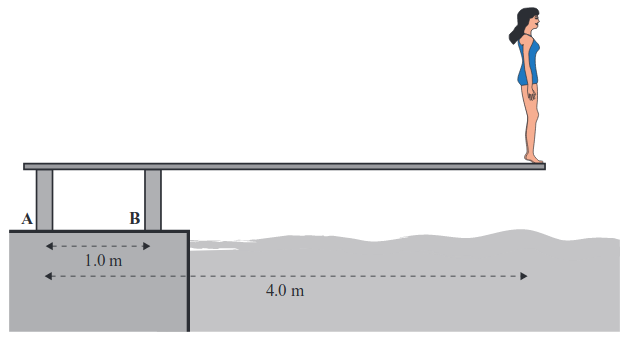
\includegraphics[width=0.4\textwidth]{nzqa20161}

      \begin{parts}
        \part Calculate the torque exerted by Sarah about support $B$.
        \part What is the direction of the force supplied by support $A$? Explain your answer.
        \part The diving board sags \SI{0.050}{\metre} when Sarah stands still on the end of the board. Assuming
              the board acts like a spring, calculate the spring constant of the board.
        \part Sarah then jumps up and lands on the board, depressing it by a \emph{further} \SI{0.20}{\metre}, before she
              dives into the water. Calculate Sarah’s speed when she lands on the board.
      \end{parts}
    \question (NZQA 2016) Sarah releases a red car, from rest, down a slope of length \SI{0.50}{\metre}. The red car accelerates steadily
              and reaches a speed of \SI{1.5}{\metre\per\second} when it gets to the bottom of the slope.
      \begin{parts}
        \part Calculate the acceleration of the red car as it moves down the slope.
        \part At the bottom of the slope, the track is flat. The red car, moving with the speed of \SI{1.5}{\metre\per\second},
              collides with a stationary blue car. The mass of the red car is \SI{0.050}{\kilo\gram}, and the mass of the blue
              car is \SI{0.040}{\kilo\gram}.
          \begin{subparts}
            \subpart If the velocity of the blue car after the collision is \SI{1.2}{\metre\per\second}, calculate the
                     velocity of the red car after the collision.
            \subpart If the duration of the collision was 0.08 seconds, calculate the average force that the red car
                     exerts on the blue car.
          \end{subparts}
      \end{parts}
    \question A car of mass $ m $ rolls from rest down a hill of height $ h $ and length $ L $. Show that when the
              car reaches the bottom it has a speed of
              \[ v = \sqrt{2gh} \]
  \end{questions}

  \section*{Section 2.6}
  Main concepts you should understand: vector components, projectiles.
  \begin{questions}
    \question Define `projectile motion'. (Describe the situations for which it is a reasonable model,
              and explain which simplifying assumptions are made.)
    \question
      \begin{parts}
        \part A ball is shot vertically upwards with a velocity of \SI{30.0}{\metre\per\second}.
          \begin{subparts}
            \subpart What maximum height does it reach?
            \subpart How long does it take for the ball to fall back to its initial height?
          \end{subparts}
        \part The ball is shot at \ang{30} to the horizontal, with the same initial speed.
          \begin{subparts}
            \subpart Draw a free body diagram showing the forces acting on the ball at the following
                  three points: (A) when it has just left the ground; (B) when it is at its peak;
                  (C) the instant before it hits the ground at the end of its flight.
            \subpart What maximum height does it reach?
            \subpart How long does it take for the ball to fall back to its initial height?
          \end{subparts}
        \part If the ball is shot at the same speed, but at \ang{45}, does its range increase
              when compared with part (b)?
      \end{parts}
    \question (NZQA 2016) During a cricket game a batsman hits the ball at an angle of
              \ang{40.0} with the ground at a velocity of \SI{20.0}{\metre\per\second}. Give
              a comprehensive explanation of the effect of the force(s) acting on the
              ball during its flight. Assume air resistance is negligible.

              In your answer you should:
              \begin{itemize}
                \item describe the horizontal motion
                \item discuss the effect of force(s) on horizontal motion
                \item describe the vertical motion
                \item discuss the effect of force(s) on vertical motion.
              \end{itemize}
    \question (NZQA 2012) Jess drops vertically onto the end of a see-saw, causing Hannah (who is standing
              at the other end) to be thrown into the air. When Jess lands on the see-saw, Hannah is thrown into
              the air at a speed of \SI{15.0}{\metre\per\second}, at an angle of \ang{70} to the horizontal.
      \begin{parts}
        \part Calculate the time that Hannah takes to reach the highest point of her trajectory.
        \part When Hannah takes off, the horizontal component of her velocity is \SI{5.1}{\metre\per\second}. State the
              size and direction of her velocity at the highest point. Explain your answer.
      \end{parts}
    \question (NZQA 2013) Hillary attempts to throw a basketball into a hoop.
      \begin{parts}
        \part Explain the effect of the force(s) acting on the ball, once it has left
              Hilary’s hand until it reaches maximum height. You may ignore the effects of air resistance.
        \part On another occasion, Hillary stands 3.0 metres from the hoop. She throws a ball with an initial
              velocity of \SI{6.5}{\metre\per\second} at an angle of \ang{60} to the horizontal. The hoop is \SI{1.35}{\metre}
              above the bottom of the ball when it is thrown initially. Carry out calculations to determine whether
              or not the ball will go through the hoop. Begin your answer by calculating the horizontal and vertical
              components of the initial velocity of the ball.
      \end{parts}
    \question Jeremy throws a ball horizontally at a speed of \SI{15.0}{\metre\per\second}. It is initially at a height of
              \SI{2.00}{\metre}. Draw a free-body diagram of force(s) acting on the ball at the instant it is thrown. How
              far does it travel?
    \question In the situation pictured below, a stunt driver wishes to shoot off the incline and land on the platform. What is
              the minimum speed the driver needs to move at in order to succeed?

              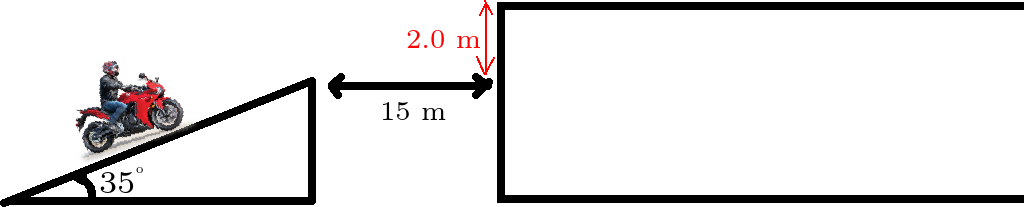
\includegraphics[width=0.4\textwidth]{motorcycle}

    \question A projectile is shot from the ground with a velocity $ u $ at an angle $ \alpha $ with the horizontal. It returns
              to the ground at a distance $ R $ from the initial point. Show that, if friction is negligible, then
              \begin{displaymath}
                R = \frac{2u^2 \sin \alpha \cos \alpha}{g};
              \end{displaymath}
              given that $ 2 \sin \alpha \cos \alpha = \sin 2\alpha $, show that the range is maximised when $ \alpha = \ang{45} $.
  \end{questions}

  \section*{Section 2.7}
  \begin{questions}
    \question In the Bohr model of the hydrogen atom, an electron is modelled as rotating in a circle (with radius \SI{0.5e-10}{\metre})
              about the positively charged nucleus of the atom.
      \begin{parts}
        \part What force furnishes the centripetal force which causes the electron to be trapped?
        \part The mass of an electron is \SI{9e-31}{\kilo\gram}, and the speed of an electron is modelled as \SI{2.3e6}{\metre\per\second}.
              How strong is the centripetal force?
        \part There is a significant issue with this model. What is it? [Hint 1: there is a conservation law being violated. Which, and why?]
        \part There is a subtle issue with the argument in (c). What is it? [Hint 2: Unpack $ \Delta E = F \Delta x $.] (Note: nonetheless, this
              argument --- when sufficiently patched up --- does disprove the Bohr model of the atom.)\footnote{See Griffiths, \emph{Intro. to Electrodynamics},
              \S11.}
      \end{parts}
    \question (NZQA 2016) A toy red car was going round a circular part of the track at a constant speed.

              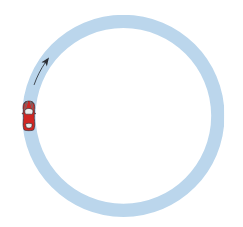
\includegraphics[width=0.4\textwidth]{nzqa20162}

      \begin{parts}
        \part Name the force acting on the car, and draw a labelled vector on the diagram above to
              show the direction of the force acting on the car at the instant shown.
        \part Discuss the effect of the force on the size and direction of the velocity of the red car.
      \end{parts}
    \question (NZQA 2012) Jess is moving in a circular path on a trapeze. When she gets to the lowest point in her
              swing, the tension force in the rope is greater than the gravity force acting on her. Draw a diagram of the
              forces acting on Jess at this time, and explain why the tension force is greater than the gravity force.
    \question (NZQA 2017) During one of her dance routines, Sally is spinning a ball above her head in a horizontal circle.
              The ball of mass \SI{0.050}{\kilo\gram} makes 5 rotations in \SI{4.0}{\second}. The length of the string
              from the ball to Sally’s hand is \SI{0.60}.
              Calculate the size of the force experienced by the ball during these rotations.
    \question A ball tied to the end of a string is swing in a vertical circle of radius $ r $ under the action of gravity.
      \begin{parts}
        \part The ball is rotating at a constant speed. Describe the acceleration felt by the ball at the top of the circle.
        \part Draw a free body diagram showing the forces acting on the ball at the top of the circle.
        \part Calculate the tension $ T $ in the string at that point.
      \end{parts}
    \question The moon orbits the Earth in an approximately circular path of radius \SI{3.8e8}{\metre}. It takes
              about 27 days to complete one circuit. What is the mass of the Earth? (Hint: draw a free body diagram.)
  \end{questions}

  \clearpage
  \section*{Formulae}
  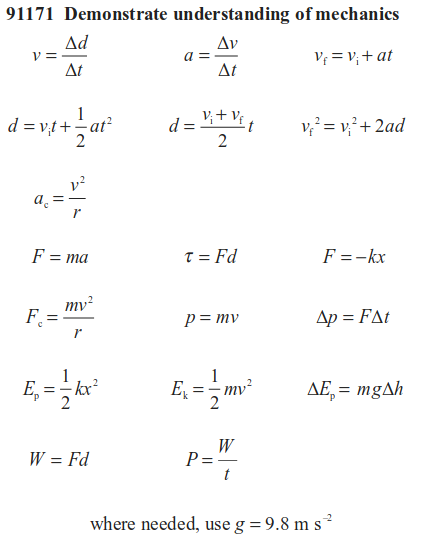
\includegraphics{mechanics}
\end{document}
